\part{Algorithmes de tri}

  \section{Tri par sélection}

    \subsection{Complexité temporelle théorique}

      \makebox[\textwidth-\parindent][s]{Le tri par sélection itère sur le tableau lors de l'appel à sa méthode principale}
      (\texttt{SelectionSorter::sort}),
      mais parcourt intégralement la partie de tableau pas encore triée
      afin de trouver l'index de l'élément le plus faible pour chacune de ces parties.
      Autrement dit, le nombre de comparaisons (et potentiellement d'échange, suivant le résultat de cette comparaison)
      est :

      \begin{align*}
       N &= n + (n - 1) + (n - 2) + ... + (n - (n-2)) + (n - (n-1)) \\
           &= \sum_{i = 1}^{n} i \\
           &= \frac{n(n-1))}{2} \\
           &= \mathcal{O}(n^2)
      \end{align*}

      On obtient donc une complexité asymptotique en $\mathcal{O}(n^2)$, c'est-à-dire une \textbf{complexité quadratique}.

    \subsection{Mesure expérimentale de la complexité temporelle}

    L'exécution de notre programme visant à mesurer la complexité temporelle du tri par sélection nous donne le
    graphe suivant :


    \begin{center}
      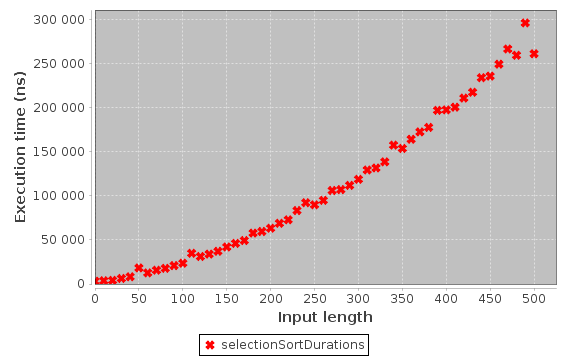
\includegraphics[width=13cm]{selectionSortTimeComplexity}
    \end{center}

    Ce graphe est cohérent avec le résultat obtenu précedemment, puisque l'on y observe une courbe de forme quadratique.

  \section{Tri à bulles}

    \subsection{Complexité temporelle théorique}

      Le nombre d'itérations réalisées par le tri à bulles dépend de l'ordre initial des éléments du tableau.
      Dans le meilleur cas (tableau déjà trié), l'algorithme n'effectue qu'un seul parcours du tableau, et a
      donc une complexité linéaire. Dans le pire cas, il le parcourt autant de fois qu'il a besoin de permuter les éléments
      du tableau, et réalise $n^2$ permutations. Il a alors une complexité quadratique.

      Cependant, sa complexité moyenne est également quadratique. En effet, le nombre d'itérations sur le tableau
      dépend du nombre de permutations nécessaire, et on peut démontrer que le nombre de permutations nécessaires pour
      un tableau initial trié dans un ordre aléatoire est en moyenne égal à $n(n-1)/4$.

    \subsection{Mesure expérimentale de la complexité temporelle}

      L'exécution de notre programme dessine le graphe suivant pour le tri à bulles :
      \begin{center}
        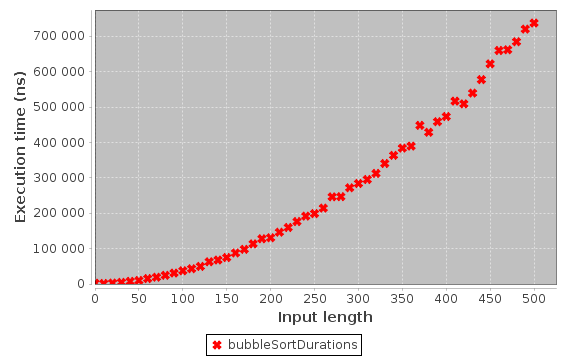
\includegraphics[width=13cm]{bubbleSortTimeComplexity}
      \end{center}

      Ce graphe est cohérent avec le résultat obtenu précedemment, puisque l'on y observe
      une courbe de forme quadratique.

  \section{Tri fusion}
    \subsection{Complexité temporelle théorique}

      Intéressons-nous tout d'abord à la fonction servant à fusionner deux sous-tableaux triées. Celle-ci
      possède une complexité en $\mathcal{O}(m + n)$, où $m$ et $n$ sont les tailles respectives des deux tableaux.
      En effet, quoi qu'il
      arrive, elle parcourra la totalité de chacun de ces deux tableaux, puisqu'elle doit comparer la première
      valeur des deux tableaux pour décider laquelle insérer dans le tableau final. Il est à noter que l'implémentation
      proposée a une complexité spatiale minimale : elle ne réalise une copie que de la première des deux parties de
      tableaux qu'elle doit fusionner, et travaille directement sur le tableau final. Autrement dit, si
      $m$ et $n$ sont les tailles
      de ces deux tableaux, la mémoire supplémentaire qu'elle nécessite pour travailler est uniquement celle occupée par
      un tableau de taille $m$.

      Puis, étudions la complexité temporelle de l'algorithme complet. Ici, on devrait trouver $n \log{}(n)$, mais c'est
      un résultat que je ne suis pas parvenu à retrouver de moi-même.

    \subsection{Mesure expérimentale de la complexité temporelle}

      L'exécution de notre programme dessine le graphe suivant pour le tri fusion :
      \begin{center}
        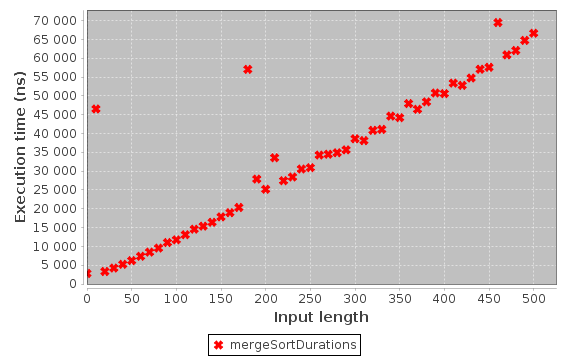
\includegraphics[width=13cm]{mergeSortTimeComplexity}
      \end{center}

      Ce graphe est cohérent avec une complexité temporelle en $n \log{}(n)$. En effet, la courbe représentative de la
      fonction $x \mapsto x \log{}(x)$ est très proche de celle d'une fonction linéaire, et nous observons effectivement ce
      type de courbe dans le graphique ci-dessus.

    \section{Tri rapide}
      \subsection{Complexité temporelle théorique}
      \subsection{Mesure expérimentale de la complexité temporelle}
        L'exécution de notre programme dessine le graphe suivant pour le tri rapide :
        \begin{center}
          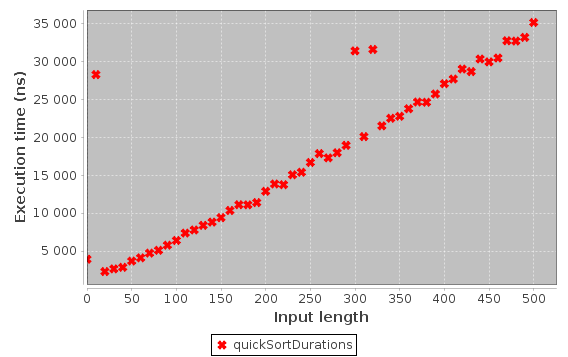
\includegraphics[width=13cm]{quickSortTimeComplexity}
        \end{center}

      Nous retrouvons ici encore un graphe cohérent avec la complexité en $n \log{} (n)$ du tri rapide.

    \section{Comparaison des différents algorithmes de tri}

      Un aspect intéressant de l'étude de la complexité temporelle des différents algorithmes est la comparaison de
      leurs performances. Le tracé de leurs temps d'exécution dans un même graphique produit le résultat suivant :

      \begin{center}
        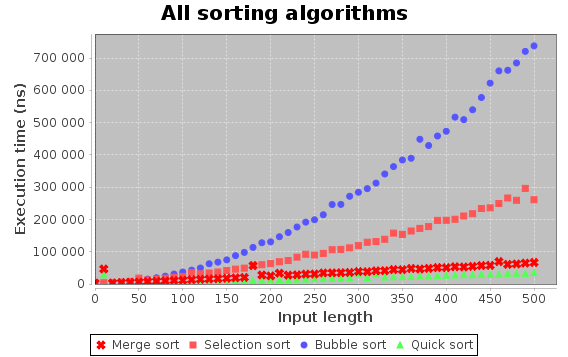
\includegraphics[width=13cm]{comparison}
      \end{center}

      Nous observons plusieurs détails intéressants sur ce graphique. Tout d'abord, on observe la large
      dispersion des courbes pour des tableaux de taille élevée.

      Nous avons observé que le tri par sélection et le tri par bulle possèdent tous deux une complexité quadratique.
      Cependant, le tri par sélection réalise $n(n-1) / 2$ itérations dans \textbf{tous} les cas, alors que le tri
       par bulle réalise en moyenne $n(n-1) / 4$ itérations. On observe une courbe pour le tri par bulle qui prend des valeurs
       approximativement égales à la moitié de celles prises par la courbe représentant les temps d'exécution du tri par
       sélection, ce qui est parfaitement normal.

       Enfin, le tri fusion et le tri rapide possèdent tous deux une complexité en $n \log{}(n)$, et ont
       donc des courbes très proches. Cependant, le tri rapide réalise toutes ses opérations en place dans le tableau initial,
       alors que le tri fusion nécessite de copier en mémoire une des deux zones à fusionner. Cette opération de copie peut
       expliquer le léger écart entre les deux courbes, en faveur du tri rapide.
